% !TeX root = ../Main-Report.tex

\chapter{Continuous Trajectory}
The enxt task was to implement a continuous trajectory between the chosen task space points from before(table \ref{tab:jspace_waypoints}), but without any full-stops at the via position. To achieve this, a cubic spline interpolation has been implemented. The joint position and velocites can be viewed in figure \ref{fig}

\begin{figure}[H]
	\centering
	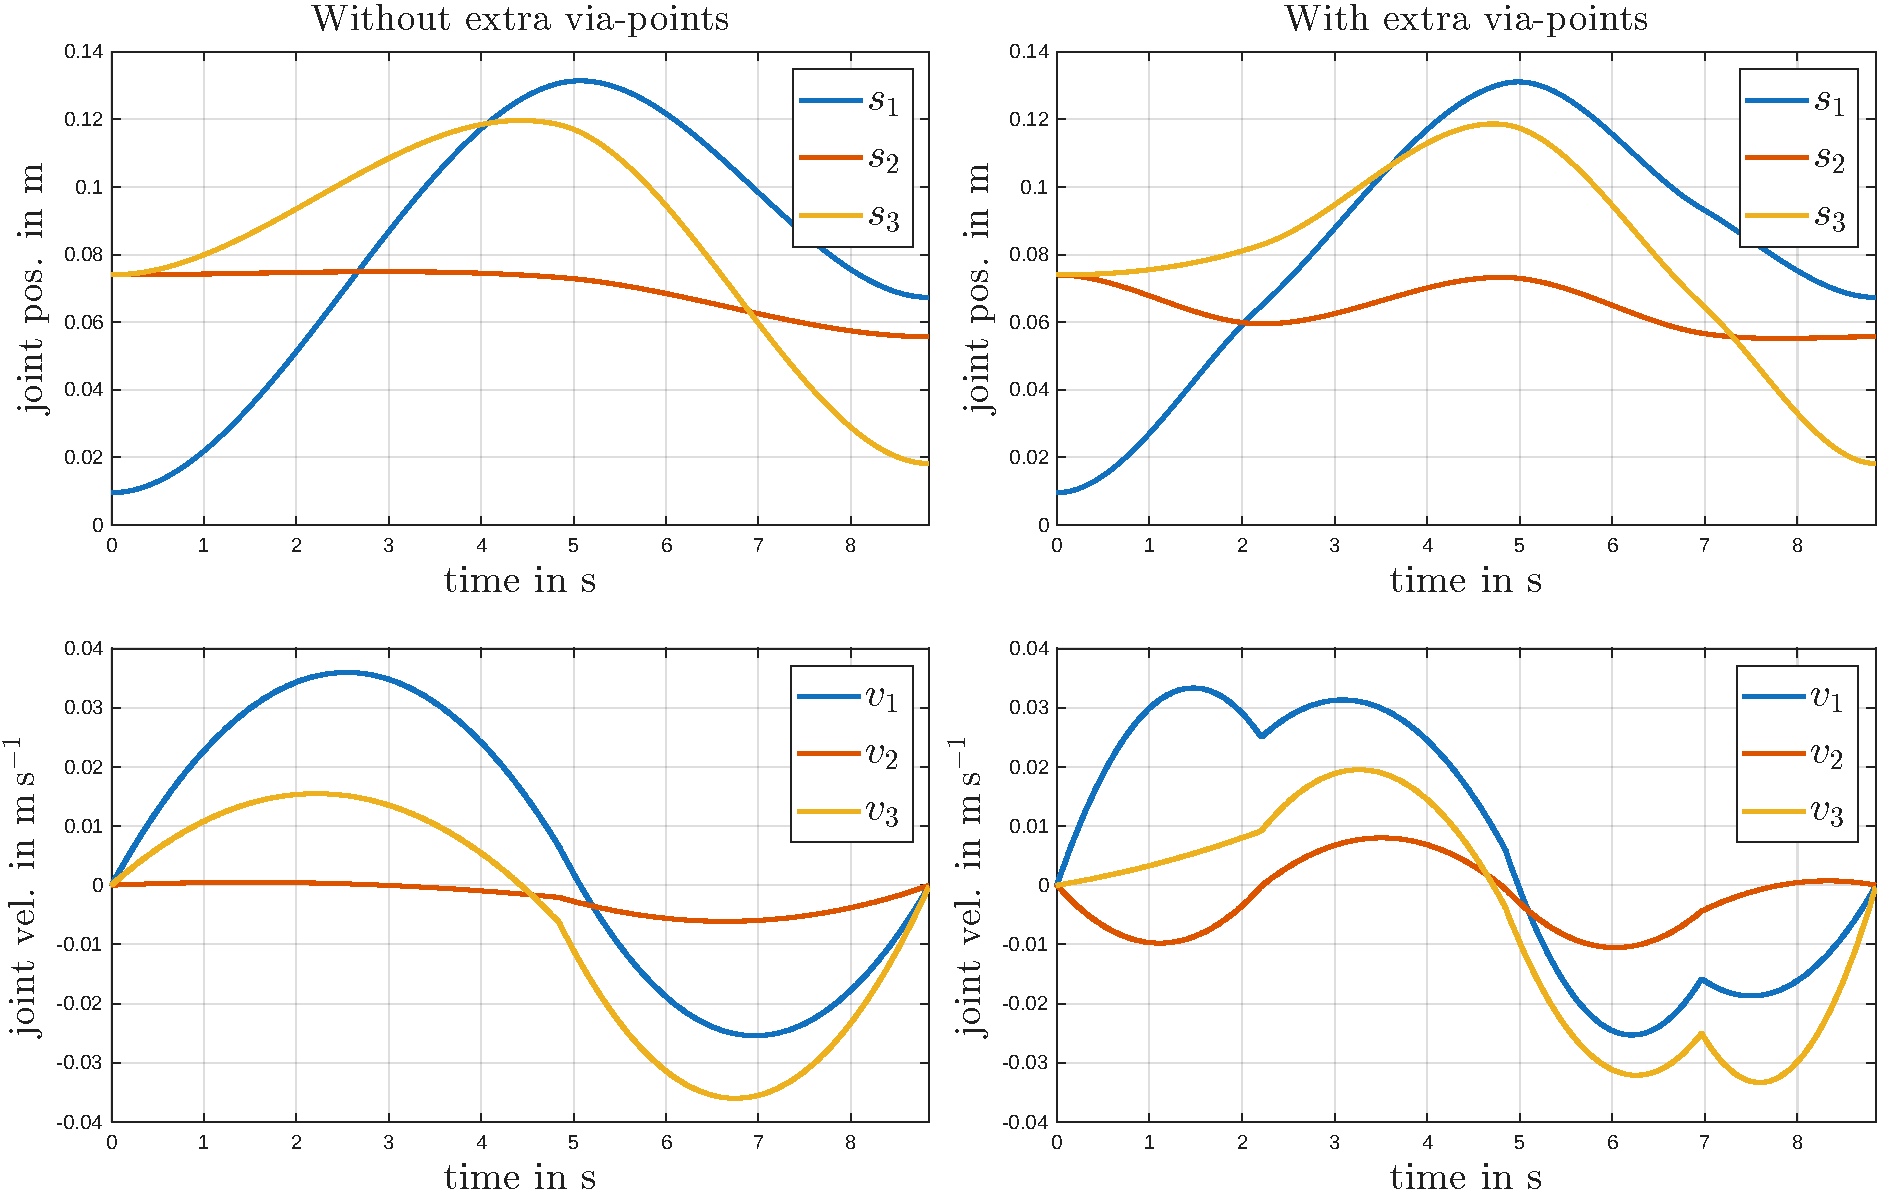
\includegraphics[width=1.0\linewidth]{cus_imgs/joint_con.pdf}
	\caption{Position and velocity of joints using a continuous trajectory, with and without extra via-points}
	\label{fig:jspace_con}
\end{figure}


\begin{figure}[H]
	\centering
	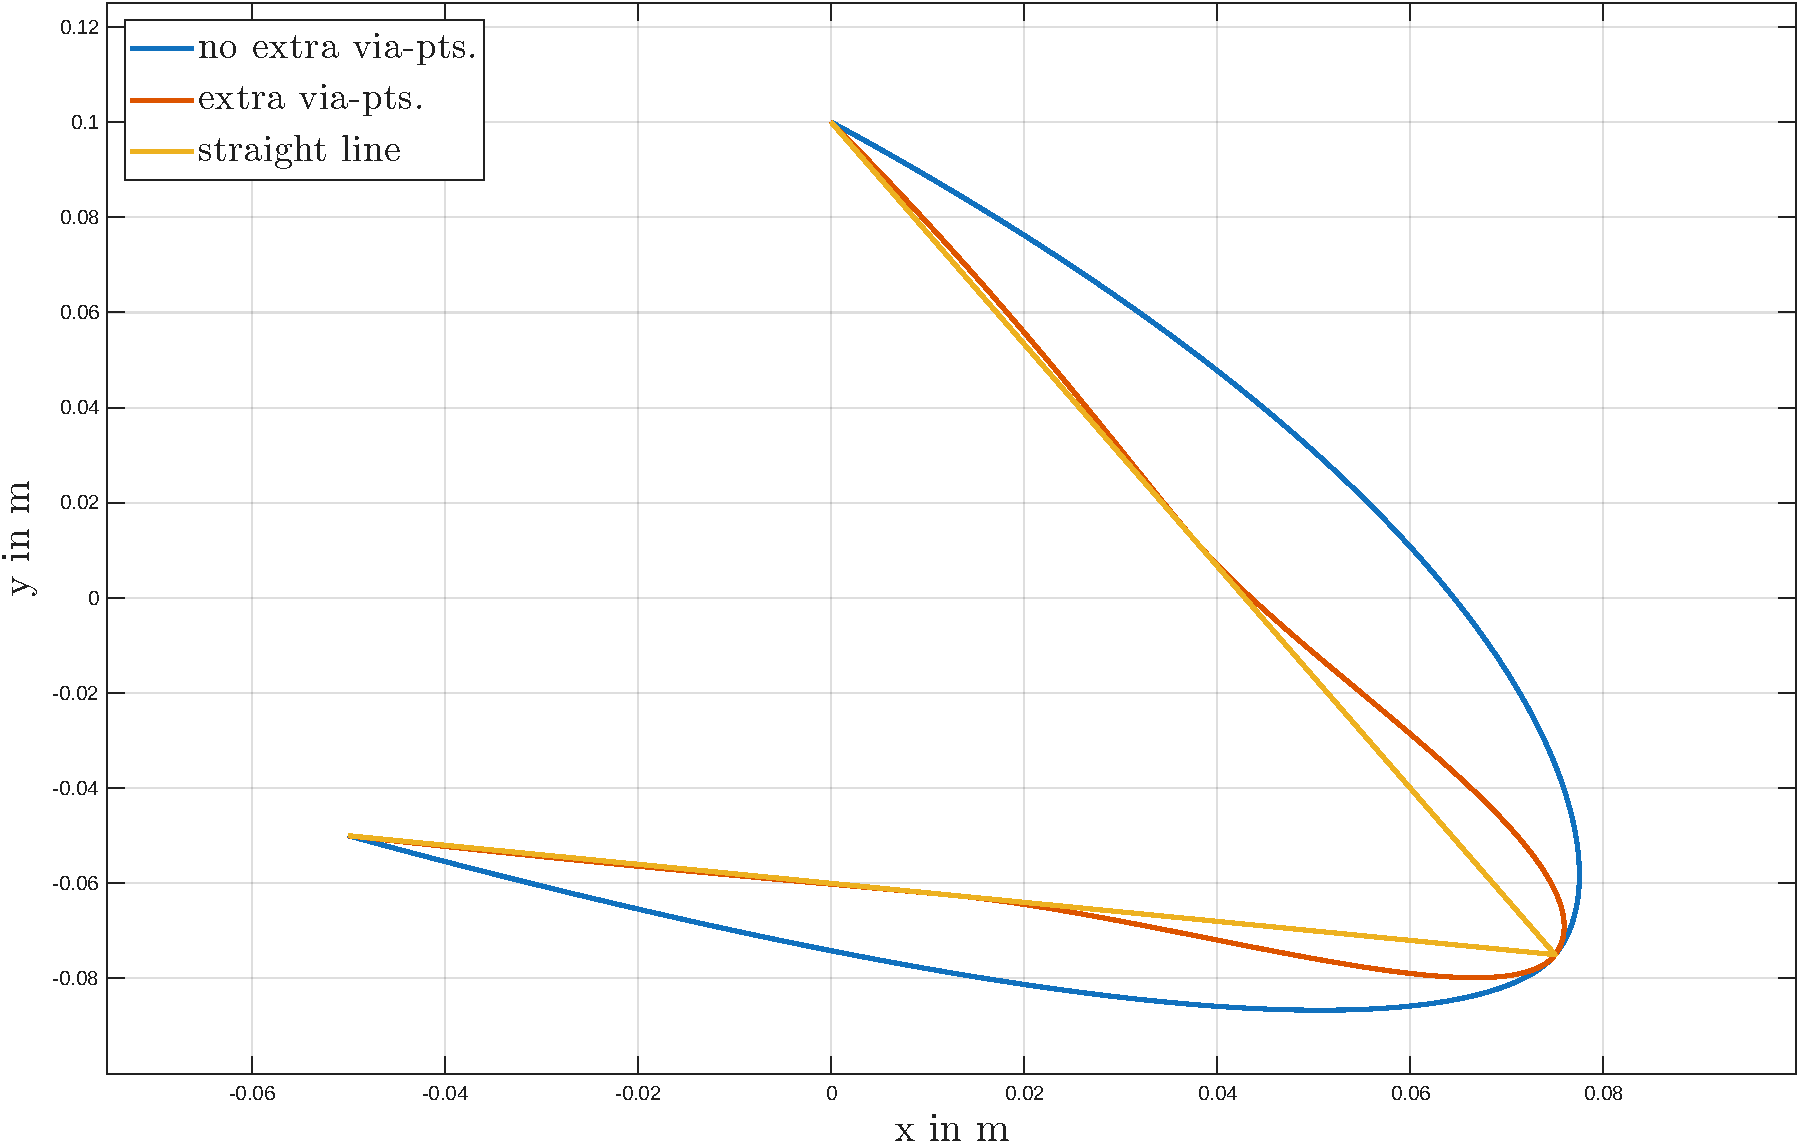
\includegraphics[width=1.0\linewidth]{cus_imgs/con_viapoints.pdf}
	\caption{End-effector $x$ and$y$ position with and without extra via-points}
	\label{fig:with_without_vias}
\end{figure}